\documentclass[a4paper,11pt]{article}

\usepackage[top=0.79in, bottom=0.79in, left=0.75in, right=0.75in]{geometry}
\setlength{\textwidth}{6.6in}
\setlength{\parindent}{1cm}

\usepackage{amsmath}
\usepackage{amssymb}
\usepackage{graphicx}
\usepackage{subfig}
\usepackage{comment}
\usepackage{booktabs}
\usepackage{multirow}
%\usepackage{color,soul}
\usepackage[usenames,dvipsnames]{xcolor}

\usepackage{pdflscape}

\usepackage{pgfplots}
\usetikzlibrary{matrix,chains,positioning,decorations.pathreplacing,arrows}

\newcommand{\fpar}[2]{\frac{\partial #1}{\partial #2}}
\def\rot#1{\rotatebox{90}{#1}}

\DeclareMathOperator{\tr}{Tr}

\renewcommand{\thefootnote}{\roman{footnote}}

\setcounter{secnumdepth}{5}
\setcounter{tocdepth}{5}

\usepackage{hyperref}

\begin{document}

\textbf{\Large{Summary of Andrew Ng's course on Machine learning}}

\tableofcontents

\newpage

\section{Summary}
\subsection{Supervised Learning}
\subsubsection{Linear Regression}
Liner regression hypothesis:\footnote{For proper notes need to expand this introductory bit: describe what and why we are doing here.}
\begin{equation}
h(x) = \sum_{j = 0} ^n \theta_j x_j = \theta^T x ,
\end{equation}
for \textcolor{OliveGreen}{$n$} features, hence \textcolor{OliveGreen}{$n$} parameters in vector \textcolor{OliveGreen}{$\theta$}, where \textcolor{OliveGreen}{$\theta_0$} is the intersect term corresponding to \textcolor{OliveGreen}{$x_0 = 0$}.

The goal of a regression problem is to fit parameters \textcolor{OliveGreen}{$\theta$}.

Ordinary least squares cost function:\footnote{Again, need a description here: why cost function, why least squares, etc.}
\begin{equation}
J \left( \theta \right) = \frac{1}{2} \sum_{i=1} ^m \left( h_\theta (x^{(i)}) - y^{(i)} \right)^2
\end{equation}
and this shall tend to zero for a good model.

\noindent\fbox{\parbox{\textwidth}{
\textbf{Aside:}

Notation tips: \textcolor{OliveGreen}{$x$} and \textcolor{OliveGreen}{$y$} are vectors, \textcolor{OliveGreen}{$x^{(i)}$} is the \textcolor{OliveGreen}{$i^{th}$} element of vector \textcolor{OliveGreen}{$x$}.\footnote{This has to be converted to proper covariant tensor notation with summation convention applied if necessary.} We do not use any special symbols (like \textcolor{OliveGreen}{$\vec{a}$} or \textcolor{OliveGreen}{$\mathbf{B}$}) to denote vectors in order not to overweight the notation.
}}

Gradient descent algorithm:
\begin{equation}
\theta_j \leftarrow \theta_j - \alpha \frac{\partial}{\partial \theta_j} J \left( \theta \right) ,
\end{equation}
where \textcolor{OliveGreen}{$\alpha$} is the learning rate.

LMS update rule (Widrow-Hoff learning rule) for a feature \textcolor{OliveGreen}{$\theta_j$}:
\begin{equation}
\theta_j \leftarrow \theta_j - \alpha \left( y^{(i)} - h_\theta \left( x^{(i)} \right) \right) x_j ^{(i)}
\end{equation}
with summation convention applied. The last term is the derivative of the cost function with respect to \textcolor{OliveGreen}{$\theta_j$}:
\begin{equation}
\frac{\partial}{\partial \theta_j} J \left( \theta \right) = \sum_{i=0} ^m \left( y^{(i)} - h_\theta \left( x^{(i)} \right) \right) x_j ^{(i)} . \label{Jdtheta}
\end{equation}

This rule has to be applied until convergence, i.e. until \textcolor{OliveGreen}{$J \rightarrow 0$}.

Define \textcolor{OliveGreen}{$X$} as a matrix of variables of size \textcolor{OliveGreen}{$n \times m$}, i.e. \textcolor{OliveGreen}{$X$} contains \textcolor{OliveGreen}{$n$} feature-vectors of \textcolor{OliveGreen}{$m$}-length each. Matrix form of \textcolor{OliveGreen}{$J \left( \theta \right)$}:
\begin{equation}
J \left( \theta \right) = \frac{1}{2} \left( X \cdot \theta - y \right)^T \left( X \cdot \theta - y \right) ,
\end{equation}
then
\begin{equation}
\nabla_\theta J \left( \theta \right) = X^T X \theta - X^T y , \label{Jnablatheta}
\end{equation}
leading to
\begin{equation}
\theta = \left( X^T \cdot X \right)^{-1} X^T y \label{theta_Normal}
\end{equation}
for \textcolor{OliveGreen}{$\nabla_\theta J \left( \theta \right)$}.
\subsubsection{Logistic Regression}
Logistic regression hypothesis:
\begin{equation}
h_\theta (x) = \frac{1}{1 + e^{-\theta^T x}}
\end{equation}
-- sigmoid function; \textcolor{OliveGreen}{$h_\theta (x)$} is the estimated probability that \textcolor{OliveGreen}{$y = 1$} on input \textcolor{OliveGreen}{$x$}, parametrised by \textcolor{OliveGreen}{$\theta$}:
\begin{equation}
h_\theta (x) = p \left( y=1 | x; \theta \right) .
\end{equation}
\textcolor{OliveGreen}{$h_\theta (x)$} is always bounded between \textcolor{OliveGreen}{$0$} and \textcolor{OliveGreen}{$1$}.

\noindent\fbox{\parbox{\textwidth}{
\textbf{Aside:}

Properties of a sigmoid function: if \textcolor{OliveGreen}{$x \rightarrow \inf$}, \textcolor{OliveGreen}{$h_\theta (x) \rightarrow 1$}; if \textcolor{OliveGreen}{$x \rightarrow -\inf$}, \textcolor{OliveGreen}{$h_\theta (x) \rightarrow 0$}, if \textcolor{OliveGreen}{$x \sim 0$}, \textcolor{OliveGreen}{$h_\theta (x) \rightarrow 0.5$}.

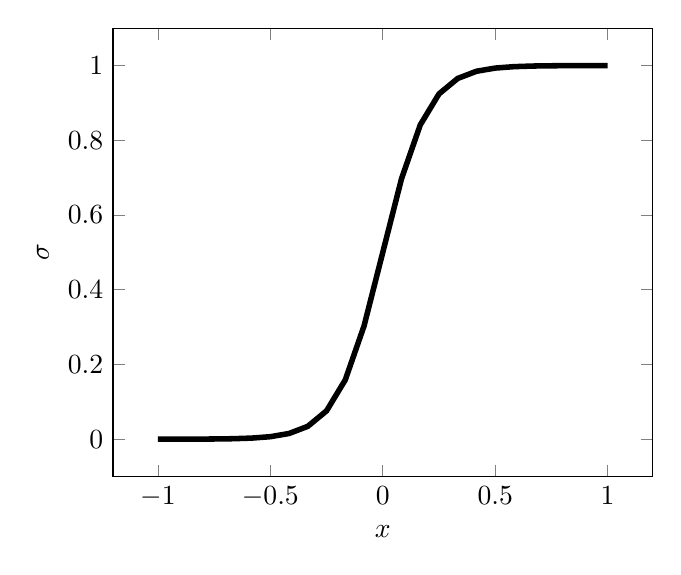
\begin{tikzpicture}
  \begin{axis}[
	domain=-1:1,
    xlabel=$x$,
    ylabel=$\sigma$
  ] 
    \addplot[color=black, line width=2] {1/(1 + e^(-10*x))}; 
  \end{axis}
\end{tikzpicture}
}}

The perceptron learning algorithm:
\begin{equation}
\theta_j \leftarrow \theta_j - \alpha \left( y^{(i)} - h_\theta \left( x^{(i)} \right) \right) x_j ^{(i)} .
\end{equation}

Cost function for logistic regression:
\begin{equation}
J \left( \theta \right) = \frac{1}{m} \sum_m \text{Cost} \left(h_\theta (x), y \right) .
\end{equation}
\begin{equation}
\text{Cost} \left(h_\theta (x), y \right) = \begin{cases}
      -\log \left(h_\theta (x) \right), & \text{if}\ y=1 \\
      -\log \left(1 - h_\theta (x) \right), & \text{if}\ y=0 .
    \end{cases}
\end{equation}
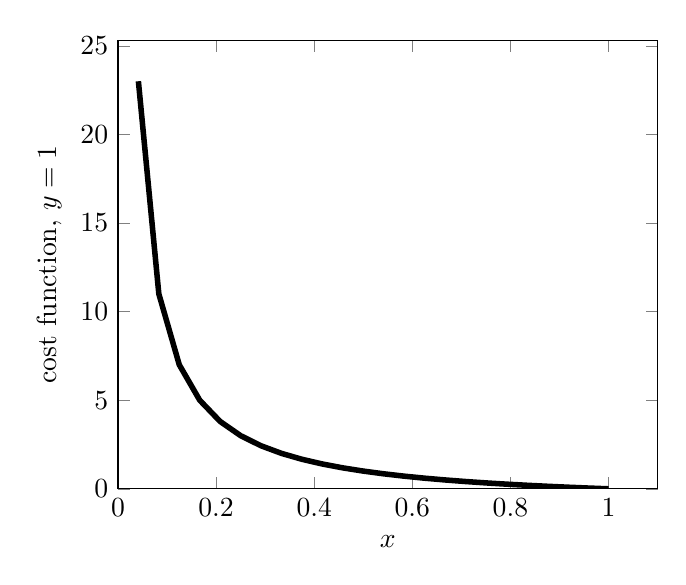
\begin{tikzpicture}
  \begin{axis}[
	domain=0:1,
	xmin=0,
	ymin=0,
    xlabel=$x$,
    ylabel={cost function, $y=1$}    
  ] 
    \addplot[color=black, line width=2] {1/x - 1}; 
  \end{axis}
\end{tikzpicture}
\hskip 5pt
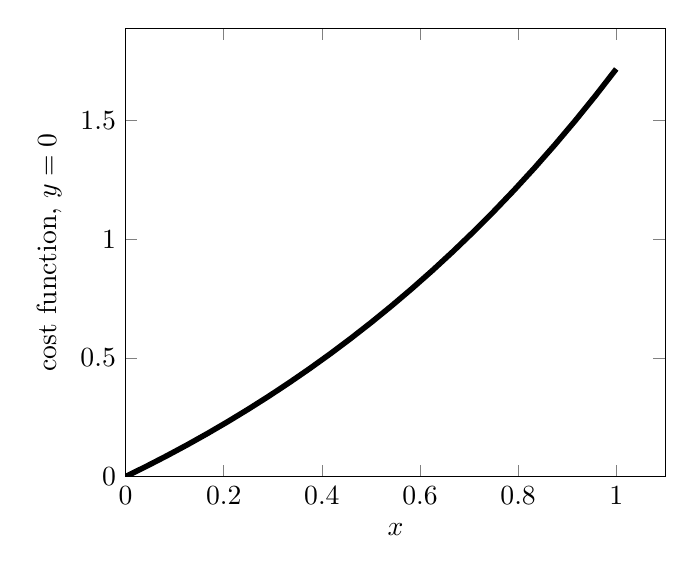
\begin{tikzpicture}
\begin{axis}[
	domain=0:1,
	xmin=0,
	ymin=0,
    xlabel=$x$,
    ylabel={cost function, $y=0$}
  ] 
    \addplot[color=black, line width=2] {e^x - 1}; 
  \end{axis}
\end{tikzpicture}
\begin{equation}
\text{Cost} \left(h_\theta (x), y \right) = -y \log \left(h_\theta (x) \right) - \left(1 - y \right) \log \left(1 - h_\theta (x) \right)
\end{equation}
\begin{equation}
J \left( \theta \right) = \frac{1}{m} \sum_{i = 1} ^m \left[ y^{(i)} \log \left(h_\theta (x^{(i)}) \right) + \left(1 - y^{(i)} \right) \log \left(1 - h_\theta (x^{(i)}) \right) \right] .
\end{equation}
\subsubsection{Regularisation}
In order to prevent an algorithm from overfitting may apply regularisation: empirically add some irregularity to the cost function.

Regularisation cost function for a linear regression:
\begin{equation}
J \left( \theta \right) = \frac{1}{2m} \sum_{i = 1} ^m \left[ h_\theta (x^{(i)}) - y^{(i)} \right]^2 + \lambda \sum_{j = 1} ^m \theta_j ^2 ,
\end{equation}
where \textcolor{OliveGreen}{$\lambda$} is the regularisation parameter.

Gradient descent:
\begin{equation}
\theta_j \leftarrow \theta_j \left(1 - \alpha\frac{\lambda}{m} \right) - \frac{\alpha}{m} \sum_{i = 1} ^m \left[ \left( h_\theta (x^{(i)}) - y^{(i)} \right) x_j ^{(i)} \right] . \label{dtheta_lambda}
\end{equation}

Normal equation under gradient descent:
\begin{equation}
\theta = \left( X^T \cdot X + \lambda L \right)^{-1} X^T y ,
\end{equation}
where
\begin{equation}
L = \begin{bmatrix}
	0 & & & & & \\
	& 1 & & & & \\
	& & 1 & & & \\
    & & & \ddots & & \\
    & & & & 1
\end{bmatrix} .
\end{equation}

The same regularisation, \textcolor{OliveGreen}{$J_\lambda = \sum\limits_{j=1} ^m \theta_j ^2$}, works for logistic regression as well.
\subsubsection{Neural Networks}
The forward propagation:

\def\layersep{2.5cm}
\begin{tikzpicture}[shorten >=1pt,->,draw=black!50, node distance=\layersep]
    \tikzstyle{every pin edge}=[<-,shorten <=1pt]
    \tikzstyle{neuron}=[circle,fill=black!25,minimum size=25pt,inner sep=0pt]
    \tikzstyle{input neuron}=[neuron, fill=green!50];
    \tikzstyle{output neuron}=[neuron, fill=red!50];
    \tikzstyle{hidden neuron}=[neuron, fill=blue!25];
    \tikzstyle{annot} = [text width=4em, text centered]

    % Draw the input layer nodes
    \foreach \name / \y in {1,...,3}
    % This is the same as writing \foreach \name / \y in {1/1,2/2,3/3,4/4}
        \node[input neuron, pin=left:$x_\y$] (I-\name) at (0,-\y) {};

    % Draw the hidden layer nodes
    \foreach \name / \y in {1,...,3}
        \path[yshift=0.cm]
            node[hidden neuron] (H-\name) at (\layersep,-\y cm) {$a_\y ^{(2)}$};

    % Draw the output layer node
    \node[output neuron,pin={[pin edge={->}]right:$h_\Theta (x)$}, right of=H-2] (O) {};

    % Connect every node in the input layer with every node in the
    % hidden layer.
    \foreach \source in {1,...,3}
        \foreach \dest in {1,...,3}
            \path (I-\source) edge (H-\dest);

    % Connect every node in the hidden layer with the output layer
    \foreach \source in {1,...,3}
        \path (H-\source) edge (O);

    % Annotate the layers
    \node[annot,above of=H-1, node distance=1cm] (hl) {Hidden layer};
    \node[annot,left of=hl] {Input layer};
    \node[annot,right of=hl] {Output layer};
\end{tikzpicture}\\
where \textcolor{OliveGreen}{$a_k ^{(l)}$} is the activation of unit \textcolor{OliveGreen}{$k$} in layer \textcolor{OliveGreen}{$l$} and \textcolor{OliveGreen}{$\Theta^{(l)}$} is the matrix of weights controlling function mapping from layer \textcolor{OliveGreen}{$l$} to \textcolor{OliveGreen}{$l+1$}; dimensions of \textcolor{OliveGreen}{$\Theta^{(l)}$} are \textcolor{OliveGreen}{$s_{l+1} \times (s_l + 1)$}.

A logistic neural net with one hidden layer can be thought of as a logistic regression with outputs of the hidden layer as inputs.

Activations are calculated via
\begin{equation}
a_1 ^{(2)} = g \left( \Theta_{10} ^{(1)} x_0 + \Theta_{11} ^{(1)} x_1 + \Theta_{12} ^{(1)} x_2 + \Theta_{13} ^{(1)} x_3 \right) ,
\end{equation}
\begin{equation}
a_2 ^{(2)} = g \left( \Theta_{20} ^{(1)} x_0 + \Theta_{21} ^{(1)} x_1 + \Theta_{22} ^{(1)} x_2 + \Theta_{23} ^{(1)} x_3 \right) ,
\end{equation}
\begin{equation}
a_3 ^{(2)} = g \left( \Theta_{30} ^{(1)} x_0 + \Theta_{31} ^{(1)} x_1 + \Theta_{32} ^{(1)} x_2 + \Theta_{33} ^{(1)} x_3 \right) ,
\end{equation}
where \textcolor{OliveGreen}{$g$} is the activation function -- a sigmoid in a case of a logistic neural net, and
\begin{equation}
h_\Theta (x) = a_1 ^{(3)} = g \left( \Theta_{10} ^{(2)} a_0 ^{(2)} + \Theta_{11} ^{(2)} a_1 ^{(2)}  + \Theta_{12} ^{(2)} a_2 ^{(2)}  + \Theta_{13} ^{(2)} a_3 ^{(2)}  \right) .
\end{equation}

Cost function for a neural network:
\begin{equation}
J \left(\Theta \right) = - \frac{1}{m} \left[ \sum_{i=1} ^m \sum_{k=1} ^K y_k ^{(i)} \log \left(h_\theta (x^{(i)}) \right)_k + \left(1 - y^{(i)} \right) \log \left(1 - h_\theta (x^{(i)}) \right)_k \right] + \frac{\lambda}{2m} \sum_{l=1} ^L \sum_{i=1} ^{s_l} \sum_{k=1} ^{s_{l+1}} \left( \Theta_{ji} ^{(l)} \right)^2 ,
\end{equation}
where \textcolor{OliveGreen}{$L$} is the total number of layers, \textcolor{OliveGreen}{$s_l$} is the number of units in layer \textcolor{OliveGreen}{$l$}, \textcolor{OliveGreen}{$K$} is the number of units in the output layer, \textcolor{OliveGreen}{$h_\Theta (x) \in \mathbb{R}^2$}, \textcolor{OliveGreen}{$\Theta_{ji} ^{(l)} \in \mathbb{R}^1$}. Note that this cost function is applicable for a logistic neural net only.

\textit{Backpropagation} gets its name from the fact that we start calculating error from the last layer.

Define $\delta_k ^{(l)}$ as an error in activation, `error' of node \textcolor{OliveGreen}{$k$} in layer \textcolor{OliveGreen}{$l$}:
\begin{equation}
\delta_k ^{(l)} = a_k ^{(l)} - y_k ,
\end{equation}
\begin{equation}
\delta_k ^{(l-1)} = \left[ \Theta_k ^{(l-1)} \right]^T \delta_k ^{(l)} . \ast g^\prime \left( z^{(l-1)} \right) ,
\end{equation}
where \textcolor{OliveGreen}{$. \ast$} is the element-wise product;
\begin{equation}
g^\prime \left( z^{(l)} \right) = a^{(l)} . \ast \left(1 - a^{(l)} \right) .
\end{equation}

For \textcolor{OliveGreen}{$\lambda = 0$}:
\begin{equation}
\frac{\partial}{\partial \Theta_{ij} ^{(l)}} J \left( \Theta \right) = a_j ^{(l)} \delta_i ^{(l)} .
\end{equation}

Backpropagation algorithm:
\begin{itemize}
\item randomly initialise weights;
\item set \textcolor{OliveGreen}{$\Delta_{ij} ^{(l)}$}, a differential of a cost function w.r.t. \textcolor{OliveGreen}{$\Theta_{ij} ^{(l)}$};
\item loop from \textcolor{OliveGreen}{$i$} to \textcolor{OliveGreen}{$m$}:
\begin{itemize}
\item[--] set \textcolor{OliveGreen}{$a^{1} = x^{(i)}$};
\item[--] perform forward propagation to compute \textcolor{OliveGreen}{$a^{(l)}$}, \textcolor{OliveGreen}{$l \in \left[2, L \right]$};
\item[--] compute \textcolor{OliveGreen}{$\delta_k ^{(L)} = a_k ^{(L)} - y_k$};
\item[--] compute \textcolor{OliveGreen}{$\delta_k ^{(L-1)}$}, etc up to \textcolor{OliveGreen}{$\delta_k ^{(2)}$};
\item[--] compute \textcolor{OliveGreen}{$\Delta_{ij} ^{(l)} \leftarrow \Delta_{ij} ^{(l)} + a_j ^{(l)} \delta_j ^{(l-1)}$};
\item[--] compute
\begin{equation}
\frac{\partial}{\partial \Theta_{ij} ^{(l)}} J \left( \Theta \right) = D_{ij} ^{(l)} = \begin{cases}
      \frac{1}{m} \Delta_{ij} ^{(l)} + \lambda \Theta_{ij} ^{(l)}, & \text{if}\ j \neq 0 \\
      \frac{1}{m} \Delta_{ij} ^{(l)}, & \text{if}\ j=0 .
    \end{cases}
\end{equation}
\end{itemize}
\end{itemize}
\subsubsection{SVM}
Support vector machine (SVM) hypothesis:
\begin{equation}
h_\theta (x) = \begin{cases}
      1, & \text{if}\ \theta^T x > 0 \\
      0, & \text{otherwise} .
    \end{cases}
\end{equation}

Cost function:
\begin{equation}
J \left( \Theta \right) = C \sum_{i=1} ^m \left[ y^{(i)} \text{cost}_1 \left(\theta^T x^{(i)} \right) + \left(1 - y^{(i)} \right) \text{cost}_0 \left(\theta^T x^{(i)} \right) \right] + \frac{1}{2} \sum_{j=1} ^n \theta_j ^2 .
\end{equation}
This is based on the cost function for a logistic regression.

In order to minimise it, one wants
\begin{equation}
\theta^T x^{(i)} \geq 1
\end{equation}
if \textcolor{OliveGreen}{$y=1$} and
\begin{equation}
\theta^T x^{(i)} \geq 1
\end{equation}
if \textcolor{OliveGreen}{$y=0$}.

Gaussian Kernel:
\begin{equation}
\kappa \left(x, l^{(i)} \right) = e^{-\frac{||x - l^{(i)}||^2}{2 \sigma^2}} ,
\end{equation}
where \textcolor{OliveGreen}{$l^{(i)}$} are `landmarks' and a kernel might be used to replace polynomials in complex boundary problems. If \textcolor{OliveGreen}{$x \approx l^{(i)}$}, then \textcolor{OliveGreen}{$\kappa \approx 1$}, if \textcolor{OliveGreen}{$x$} is far from \textcolor{OliveGreen}{$l^{(i)}$}, then \textcolor{OliveGreen}{$\kappa \approx 0$}. I.e. the SVM would predict \textcolor{OliveGreen}{$y=1$} near \textcolor{OliveGreen}{$l^{(i)}$} and \textcolor{OliveGreen}{$y=0$} far from them. One often chooses \textcolor{OliveGreen}{$l^{(i)}$} to correspond to \textcolor{OliveGreen}{$x^{(i)}$} and so on and the kernel then goes over all of them.

SVM parameter:
\begin{equation}
C = \frac{1}{\lambda} ,
\end{equation}
hence
\begin{itemize}
\item large \textcolor{OliveGreen}{$C$} $\rightarrow$ small \textcolor{OliveGreen}{$\lambda$}: lower \textcolor{Red}{bias}, lower \textcolor{Green}{variance};
\item small \textcolor{OliveGreen}{$C$} $\rightarrow$ large \textcolor{OliveGreen}{$\lambda$}: higher \textcolor{Red}{bias}, higher \textcolor{Green}{variance};
\item large \textcolor{OliveGreen}{$\sigma^2$}: higher \textcolor{Red}{bias}, lower \textcolor{Green}{variance};
\item small \textcolor{OliveGreen}{$\sigma^2$}: lower \textcolor{Red}{bias}, higher \textcolor{Green}{variance}.
\end{itemize}

So one needs to choose \textcolor{OliveGreen}{$C$} and specify a kernel: linear, Gaussian, etc. Other possible kernels (that satisfy Mercer's theorem\footnote{The theorem itself is far beyond the scope.}):
\begin{itemize}
\item polynomial:
\begin{equation}
\kappa \left(x, l \right) = \left(x^T l + K \right)^n ;
\end{equation}
\item string kernel;
\item chi-square kernel;
\item histogram intersection kernel.
\end{itemize}
\subsection{Analysing Classification Algorithms}
\subsubsection{Misclassification Error}
Plotting \textcolor{OliveGreen}{$J \left( \Theta \right)$} against number of iterations may help.

Misclassification error:
\begin{equation}
\epsilon \left( h_\theta (x) , y \right) = \begin{cases}
      1, & \text{if}\ h_\theta (x) \geq 0.5\ \text{and}\ y=0\ \text{or}\ h_\theta (x) < 0.5\ \text{and}\ y=1 \\
      0, & \text{otherwise} ,
    \end{cases}
\end{equation}
and the average test error is then
\begin{equation}
T_\epsilon = \frac{1}{m_{test}} \sum_{i=1} ^{m_{test}} \epsilon \left( h_\theta \left(x_{test} ^{(i)}\right) , y_{test} ^{(i)} \right) .
\end{equation}

\subsubsection{Train, Validation and Test Sets}
A useful validation technique might be splitting the dataset on the train, validation and test sets if one wants to choose the best model out of several. Then
\begin{itemize}
\item train the set of models;
\item check them with the validation set;
\item pick the best and feed test set to it to find the generalised error.
\end{itemize}

\subsubsection{Bias vs Overfit}
Bias vs overfit:
\begin{itemize}
\item Bias (underfit):
\begin{equation}
J_{train} \left( \theta \right) \rightarrow \text{high} ,
\end{equation}
\begin{equation}
J_{cv} \left( \theta \right) \approx J_{train} \left( \theta \right) .
\end{equation}
\item Variance (overfit):
\begin{equation}
J_{train} \left( \theta \right) \rightarrow \text{low} ,
\end{equation}
\begin{equation}
J_{cv} \left( \theta \right) \geq J_{train} \left( \theta \right) .
\end{equation}
\end{itemize}

A learning curve is a plot of error against the training set size for a given model. Learning curves for high bias and high variance:

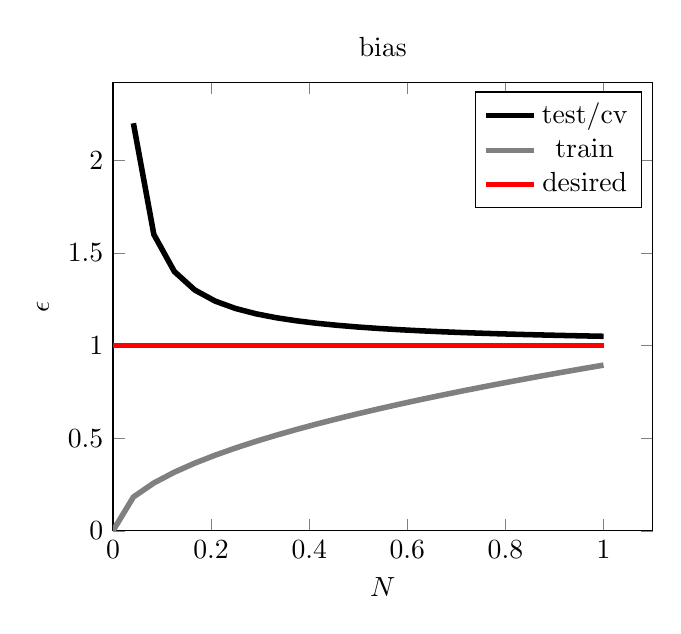
\begin{tikzpicture}
  \begin{axis}[
	title={bias},
	domain=0:1,
	xmin=0,
	ymin=0,
    xlabel=$N$,
    ylabel={$\epsilon$}    
  ] 
    \addplot[color=black, line width=2] {0.05/x + 1};
    \addlegendentry{test/cv}
    \addplot[color=gray, line width=2] {0.4*sqrt(5*x)};
    \addlegendentry{train}
    \addplot[color=red, line width=2] {1};
    \addlegendentry{desired}
  \end{axis}
\end{tikzpicture}
\hskip 5pt
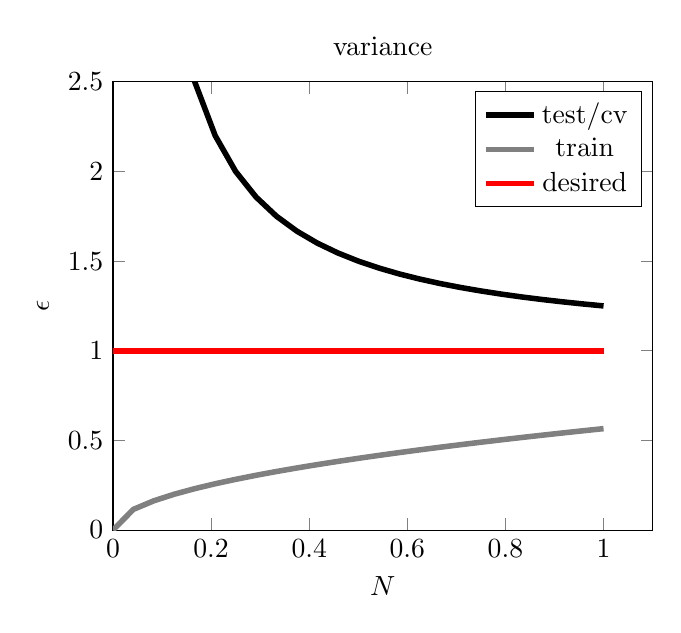
\begin{tikzpicture}
\begin{axis}[
	title={variance},
	domain=0:1,
	xmin=0,
	ymin=0,
	ymax=2.5,
    xlabel=$N$,
    ylabel={$\epsilon$}  
  ] 
    \addplot[color=black, line width=2] {0.25/x + 1};
    \addlegendentry{test/cv}
    \addplot[color=gray, line width=2] {0.4*sqrt(2*x)};
    \addlegendentry{train}
    \addplot[color=red, line width=2] {1};
    \addlegendentry{desired}
  \end{axis}
\end{tikzpicture}

Summary of potential improvements of a model:
\begin{itemize}
\item get more training examples $\rightarrow$ fixes high \textcolor{Green}{variance};
\item try smaller set of features $\rightarrow$ fixes high \textcolor{Green}{variance};
\item try additional features $\rightarrow$ fixes high \textcolor{Red}{bias};
\item try adding polynomial features $\rightarrow$ fixes high \textcolor{Red}{bias};
\item try decreasing \textcolor{OliveGreen}{$\lambda$} $\rightarrow$ fixes high \textcolor{Red}{bias};
\item try increasing \textcolor{OliveGreen}{$\lambda$} $\rightarrow$ fixes high \textcolor{Green}{variance}.
\end{itemize}

An imbalanced dataset is also called `a dataset with skewed classes'.

\subsubsection{Prediction Table}
Prediction table:

\vspace{0.5cm}
\begin{tabular}{c c | c | c |}
\multirow{4}{*}{\rot{\rlap{\hspace{-1cm}\small{Predicted class}}}} & & \multicolumn{2}{c}{ Actual class}\\\cline{3-4}
& & $1$ & $0$ \\\cline{2-4}
& $1$ & \textcolor{Blue}{True positives} & \textcolor{Red}{False positives} \\\cline{2-4}
& $0$ & \textcolor{Purple}{False negatives} & \textcolor{Green}{True negatives}\\\cline{2-4}
\end{tabular}

\vspace{0.5cm}
Precision:
\begin{equation}
P = \frac{\text{True positives}}{\text{Predicted positives}} = \frac{\textcolor{Blue}{\text{TP}}}{\textcolor{Blue}{\text{TP}} + \textcolor{Red}{\text{FP}}} .
\end{equation}

Recall:
\begin{equation}
R = \frac{\text{True positives}}{\text{Actual positives}} = \frac{\textcolor{Blue}{\text{TP}}}{\textcolor{Blue}{\text{TP}} + \textcolor{Purple}{\text{FN}}} .
\end{equation}

$F$ (or $F_1$) score:
\begin{equation}
F_1 = 2 \frac{P R}{P + R} .
\end{equation}
\subsection{Unsupervised Learning}
\subsubsection{Clustering}
K-means clustering algorithm:
\begin{itemize}
\item assign centroids;
\item move centroids;
\item repeat until convergence.
\end{itemize}

Cost function based on LMS:
\begin{equation}
J \left( C^{(1)}, \ldots , C^{(m)}, \mu_1 , \ldots , \mu_k \right) = \frac{1}{m} \sum_{i=1} ^m \left| \left| x^{(i)} - \mu_{c (i)} \right| \right|^2 ,
\end{equation}
where \textcolor{OliveGreen}{$C^{(i)}$} is the index of cluster to which example \textcolor{OliveGreen}{$x^{(i)}$} is currently assigned and \textcolor{OliveGreen}{$\mu_{c (i)}$} is the cluster centroid.
\subsubsection{Principal Component Analysis}
Principal Component Analysis (PCA): reduce dimensions and find a direction (plane or a hyperplane) that minimises the projection error.

PCA algorithm:
\begin{itemize}
\item normalise the data;
\item compute the covariance matrix:
\begin{equation}
\Sigma = \frac{1}{m} \sum_{j = 1} ^n X_j X_j ^T = \frac{1}{m} X^T X ,
\end{equation}
where \textcolor{OliveGreen}{$\Sigma$} is \textcolor{OliveGreen}{$n \times n$} matrix;
\item compute the eigenvectors of \textcolor{OliveGreen}{$\Sigma$} via singular value decomposition;
\item take first \textcolor{OliveGreen}{$k$} eigenvalues and transpose them;
\item multiply them by \textcolor{OliveGreen}{$X$}.
\end{itemize}

A typical choice of the number of the principal components retained is the minimal number that retains `99\%' of the variance:
\begin{equation}
\frac{\frac{1}{m}\sum\limits_{i = 1} ^m \left| \left| x^{(i)} - x_{\text{approx}} ^{(i)} \right| \right|^2}{\frac{1}{m}\sum\limits_{i = 1} ^m \left| \left| x^{(i)} \right| \right|^2} \leq 0.01 .
\end{equation}

Major applications of PCA is the speedup of a supervised learning algorithm or better visualisation.
\subsection{Anomaly Detection}
For a Gaussian distribution define:
\begin{equation}
\mu_j = \frac{1}{m} \sum_{i = 1} ^m x_j ^{(i)} ,
\end{equation}
\begin{equation}
\sigma_j ^2 = \frac{1}{m} \sum_{i = 1} ^m \left(x_j ^{(i)} \mu_j \right)^2 ,
\end{equation}
\begin{equation}
p (x) = \prod_{j=1} ^n p \left( x_j ; \mu_j \sigma_j ^2 \right) = \prod_{j=1} ^n \frac{1}{\sqrt{2\pi} \sigma_j} e^{-\frac{(x_j - \mu_j)^2}{2 \sigma_j ^2}} ,
\end{equation}
where \textcolor{OliveGreen}{$j$} is the number of features and \textcolor{OliveGreen}{$i$} is the number of elements in each feature-vector.

This Gaussian distribution is used for anomaly detection:
\begin{equation}
y = \begin{cases}
      1, & \text{if}\ p(x) \leq \varepsilon \\
      0, & \text{if}\ p(x) > \varepsilon\ \text{-- normal} .
    \end{cases}
\end{equation}

Then one can choose value of \textcolor{OliveGreen}{$\varepsilon$} that minimises F-score.

\subsection{Collaborative Filtering}
\textbf{Note}: this is based on an example, hence not a general formulation.

Cost function:
\begin{equation}
J \left( \theta^{(1)}, \ldots , \theta^{(n_u)} \right) = \frac{1}{2} \sum_{j=1} ^{n_u} \sum_{i:r(i,j)=1} \left( \left(\theta^{(j)} \right)^T x^{(i)} - y^{(i,j)} \right)^2 + \frac{\lambda}{2} \sum_{j=1} ^{n_u} \sum_{k=1} ^n \left(\theta^{(j)} _k \right)^2 ,
\end{equation}
where \textcolor{OliveGreen}{$i$} is the number of `movies', \textcolor{OliveGreen}{$j$} is the number of `users', \textcolor{OliveGreen}{$r(i,j)$} is a binary function denoting if a `user' rated a `movie', \textcolor{OliveGreen}{$x^{(i)}$} -- features of a `movie' and \textcolor{OliveGreen}{$y^{(i,j)}$} -- score of a `movie' \textcolor{OliveGreen}{$i$} according to `user' \textcolor{OliveGreen}{$j$} for an example of an IMDB-like system.

Gradient descent update:
\begin{equation}
\theta_k ^{(j)} \leftarrow \theta_k ^{(j)} - \alpha \sum_{i:r(i,j)=1} \left(\left(\theta^{(j)} \right)^T x^{(i)} - y^{(i,j)} \right) x_k ^{(i)}
\end{equation}
for \textcolor{OliveGreen}{$k=0$} and
\begin{equation}
\theta_k ^{(j)} \leftarrow \theta_k ^{(j)} - \alpha \left( \sum_{i:r(i,j)=1} \left(\left(\theta^{(j)} \right)^T x^{(i)} - y^{(i,j)} \right) x_k ^{(i)} + \lambda \theta_k ^{(k)} \right)
\end{equation}
for \textcolor{OliveGreen}{$k \neq 0$}.

Collaborative filtering algorithm:
\begin{itemize}
\item Initialise \textcolor{OliveGreen}{$x^{(1)}, \ldots, x^{(n_m)}, \theta^{(1)}, \ldots, \theta^{(n_u)}$} to small random values.
\item Minimise \textcolor{OliveGreen}{$J \left( x, \theta \right)$} using gradient descent (or any other algorithm).
\item For a `user' with parameters \textcolor{OliveGreen}{$\theta$} and a `movie' with (learned) features \textcolor{OliveGreen}{$x$}, predict a rating of \textcolor{OliveGreen}{$\theta^T x$}.
\end{itemize}
\subsection{Other Optimisation Algorithms}
Other algorithms to find \textcolor{OliveGreen}{$\theta$} (for large datasets):
\begin{itemize}
\item stochastic gradient descent;
\item mini-batch gradient descent.
\end{itemize}

In order to check convergence of the stochastic gradient descent one may plot \textcolor{OliveGreen}{$\text{cost} \left( \theta , \left(x^{(i)}, y^{(i)} \right) \right)$} averaged over the last 1000 (say) iterations.

If the algorithm is diverging -- use smaller \textcolor{OliveGreen}{$\alpha$}. It doesn't have to be constant:
\begin{equation}
\alpha = \frac{c_1}{i + c_2} ,
\end{equation}
where \textcolor{OliveGreen}{$i$} is the iteration number.

One may apply map reduce for data parallelisation.
\subsection{Backpropagation*}
This is a very short summary of another Andrew Ng's course.
\subsubsection{Notation and Definitions}
Define a single entry as \textcolor{OliveGreen}{$(x, y)$}, with \textcolor{OliveGreen}{$x$} being a vector,
\begin{equation}
x \in \mathbb{R}^m ,
\end{equation}
where \textcolor{OliveGreen}{$m$} is the number of training examples, hence \textcolor{OliveGreen}{$x^{(i)}$} is the \textcolor{OliveGreen}{$i^{th}$} example in a dataset and
\begin{equation}
y \in \left\lbrace 0, 1 \right\rbrace .
\end{equation}

For \textcolor{OliveGreen}{$n$} features define
\begin{equation}
X \in \mathbb{R}^{n \times m}
\end{equation}
-- an \textcolor{OliveGreen}{$n \times m$} matrix with \textcolor{OliveGreen}{$n$} rows and \textcolor{OliveGreen}{$m$} columns, where each row corresponds to a feature. Also
\begin{equation}
Y \in \mathbb{R}^{1 \times m}
\end{equation}
-- a \textcolor{OliveGreen}{$1 \times m$} matrix or just a row-vector.

Loss function is a cost function for a simple example.
\subsubsection{Activation Functions}
Define \textcolor{OliveGreen}{$a^{[l]}_k$} to be an activation of a node \textcolor{OliveGreen}{$k$} in layer \textcolor{OliveGreen}{$l$}.

In oppose to our previous convention, define
\begin{equation}
\theta = w + b ,
\end{equation}
where \textcolor{OliveGreen}{$b$} stands for \textcolor{OliveGreen}{$\theta_0$}, and \textcolor{OliveGreen}{$w$} is a vector of other \textcolor{OliveGreen}{$\theta$}-coefficients or weights.

Identity activation is just a linear function. It is used only for a regression problem approached by a neural net.

Sigmoid activation:
\begin{equation}
g(z) = \frac{1}{1 + e^{-z}} = a,
\end{equation}
where
\begin{equation}
z = w^T x + b .
\end{equation}

Sigmoid's derivative:
\begin{equation}
g^\prime (z) = a^\prime = a(1-a) .
\end{equation}

ReLU activation:
\begin{equation}
g(z) = \max \left( 0 , z \right) ,
\end{equation}
it's derivative:
\begin{equation}
g^\prime (z) = \begin{cases}
      0, & \text{if}\ z < 0 \\
      1, & \text{if}\ z \geq 0 ,
    \end{cases}
\end{equation}
although technically \textcolor{OliveGreen}{$z=0$} case is not defined.

Leaking ReLU activation:
\begin{equation}
g(z) = \max \left( \xi z , z \right) ,
\end{equation}
where \textcolor{OliveGreen}{$\xi$} is a small number, usually \textcolor{OliveGreen}{$\xi = 0.01$}.

Tanh activation:
\begin{equation}
g(z) = \tanh (z) = a,
\end{equation}
it's derivative:
\begin{equation}
g^\prime (z) = 1 - a^2 .
\end{equation}
\subsubsection{Propagations}
Carrying on with our definition of \textcolor{OliveGreen}{$X$}, similarly define \textcolor{OliveGreen}{$W$}, \textcolor{OliveGreen}{$A$} and \textcolor{OliveGreen}{$Z$}.

Forward propagation. For a layer \textcolor{OliveGreen}{$l$}:
\begin{equation}
Z^{[l]} = W^{[l]} A^{[l]} + b^{[l]} ,
\end{equation}
\begin{equation}
A^{[l]} = g \left( Z^{[l]} \right) ,
\end{equation}
\begin{equation}
A^{[0]} = X ,
\end{equation}
where \textcolor{OliveGreen}{$W^{[l]}$} is the weights matrix for a layer \textcolor{OliveGreen}{$l$}.

One has to be careful with dimensions now:
\begin{equation}
\left[W^{[l]} \right] = \left(N^{[l]} , N^{[l-1]} \right) ,
\end{equation}
\begin{equation}
\left[b^{[l]} \right] = \left(N^{[l]} , 1\right) ,
\end{equation}
\begin{equation}
\left[Z^{[l]} \right] = \left(N^{[l]} , m \right) ,
\end{equation}
\begin{equation}
\left[A^{[l]} \right] = \left(N^{[l]} , m \right) ,
\end{equation}
\begin{equation}
\left[X^{[l]} \right] = \left(N^{[0]} , m \right) ,
\end{equation}
where \textcolor{OliveGreen}{$N^{[l]}$} is the number of nodes in layer \textcolor{OliveGreen}{$l$}.

To shorthand notation define:
\begin{equation}
dW = \frac{\partial J}{\partial W} ,
\end{equation}
\begin{equation}
dZ = g^\prime \left(Z \right) ,
\end{equation}
etc.

Backpropagation:
\begin{equation}
d W^{[l]} = \frac{1}{m} d Z^{[l]} A^{[l-1] T} ,
\end{equation}
\begin{equation}
db^{[l]} = \frac{1}{m} \sum_{i=1} ^m d Z^{[l] (i)} ,
\end{equation}
\begin{equation}
d A^{[l-1]} = W^{[l]T} dZ^{[l]} ,
\end{equation}
\begin{equation}
dZ^{[l]} = dA^{[l]} \ast g^\prime \left( Z^{[l] (i)} \right) .
\end{equation}
\subsection{Tips and Tricks for Neural Networks*}
Train / dev / test split:
\begin{itemize}
\item `small data': 60/20/20 -- tens of thousands;
\item `big data': 98/1/1 -- like really big data -- millions.
\end{itemize}

Make sure that train and test sets come from the same distribution.

High variance: dev (test) set error $\gg$ train set error.

High bias: both test and train set errors are high.

High bias and high variance: both errors are high and error of the test set is $\gg$ than the error of the train set.

Basic recipe:
\begin{itemize}
\item high bias? $\rightarrow$ Bigger network, tune layers, switch architecture;
\item high variance? $\rightarrow$ More data, Regularisation, switch architecture.
\end{itemize}

Regularisations:
\begin{itemize}
\item \textcolor{OliveGreen}{$L_1$} regularisation:
\begin{equation}
J \left( w , b \right) = \frac{1}{m} \sum_{i=1} ^m \mathcal{L} \left(\hat{y}^{(i)} , y^{(i)} \right) + \frac{\lambda}{2m} \sum_{j=1} ^{n_x} \left| w \right| ;
\end{equation}
\item \textcolor{OliveGreen}{$L_2$} regularisation:
\begin{equation}
J \left( w , b \right) = \frac{1}{m} \sum_{i=1} ^m \mathcal{L} \left(\hat{y}^{(i)} , y^{(i)} \right) + \frac{\lambda}{2m} \sum_{j=1} ^{n_x} \left| w \right|^2 ,
\end{equation}
\end{itemize}
where \textcolor{OliveGreen}{$\hat{y} = h_\theta \left( x \right)$} is the predicted value.

\textcolor{OliveGreen}{$L_1$} regularisation gives quite sparse \textcolor{OliveGreen}{$w$} in the end.

Redefine \textcolor{OliveGreen}{$L_2$} for a Neural Net:
\begin{equation}
J \left( w^{[l]} , b^{[l]}, \ldots , w^{[L]} , b^{[L]} \right) = \frac{1}{m} \sum_{i=1} ^m \mathcal{L} \left(\hat{y}^{(i)} , y^{(i)} \right) + \frac{\lambda}{2m} \sum_{l=1} ^{L} \left| w^{[l]} \right|^2 _F ,
\end{equation}
where \textcolor{OliveGreen}{$\left| w^{[l]} \right|^2 _F$} is the Forbenius norm:
\begin{equation}
\left| w^{[l]} \right|^2 _F = \sum_{i=1} ^{[l]} \sum_{j=1} ^{[l-1]} \left(w_{i,j} ^{[l]} \right)^2 .
\end{equation}

Update rule:
\begin{equation}
w^{[L]} \leftarrow \left(1 - \frac{\alpha \lambda}{m} \right) w^{[L]} - \alpha dW^{[L]} _{backprop} .
\end{equation}

Other regularisation methods:
\begin{itemize}
\item dropout regularisation: randomly knock out some nodes $\rightarrow$ have to spread out weights $\rightarrow$ shrink weights; new parameters: keep-prob, this might be different for different layers; it's highly used in computer vision as you often don't have enough data;
\item data augmentation -- again, good for computer vision;
\item early stopping (i.e. stop when the curves on the plot start diverging), but it has its caveats:

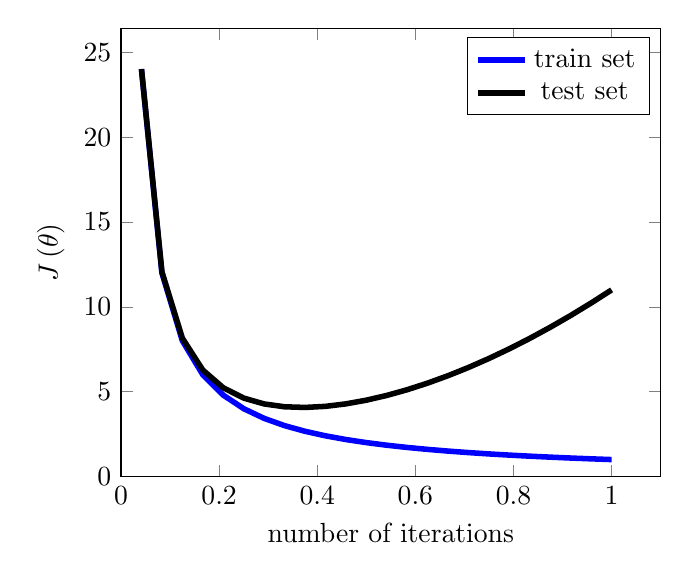
\begin{tikzpicture}
  \begin{axis}[
	domain=0:1,
	xmin=0,
	ymin=0,
    xlabel=number of iterations,
    ylabel={$J \left( \theta \right)$}    
  ] 
    \addplot[color=blue, line width=2] {1/x };
    \addlegendentry{train set}
    \addplot[color=black, line width=2] {1/x + 10*x^2};
    \addlegendentry{test set}
  \end{axis}
\end{tikzpicture}
\end{itemize}

Normalisation. Mean:
\begin{equation}
\mu = \frac{1}{m} \sum_{i=1} ^m x^{(i)} ,
\end{equation}
hence \textcolor{OliveGreen}{$x \rightarrow x - \mu$}, normal variance:
\begin{equation}
\sigma^2 = \frac{1}{m} \sum_{i=1} ^m x^{(i)^2} ,
\end{equation}
hence \textcolor{OliveGreen}{$x \rightarrow \frac{x}{\sigma^2}$}.

If use these, then use the same \textcolor{OliveGreen}{$\mu$} and \textcolor{OliveGreen}{$\sigma$} for both train and test sets.

Normalisation usually helps to speed up gradient descent.

In general, for large \textcolor{OliveGreen}{$n$} one wants small \textcolor{OliveGreen}{$w_j$}, so in random initialisation of weights one may multiply each entry by \textcolor{OliveGreen}{$\sqrt{\frac{2}{n^{[l-1]}}}$}, or \textcolor{OliveGreen}{$\sqrt{\frac{1}{n^{[l-1]}}}$}, or \textcolor{OliveGreen}{$\sqrt{\frac{2}{n^{[l-1]}+N^{[l]}}}$}.

Mini-batch gradient descent. Extreme cases:
\begin{itemize}
\item mini-batch size $=$ \textcolor{OliveGreen}{$m$}: Batch gradient descent;
\item mini-batch size $=$ \textcolor{OliveGreen}{$1$}: Stochastic gradient descent.
\end{itemize}

Stochastic gradient descent never converges, but oscillates around the minima. And you loose all the speed-up from vectorisation.

For a small training set (\textcolor{OliveGreen}{$m \leq 2000$}) use batch gradient descent.

Typical mini-batch sizes: \textcolor{OliveGreen}{$2^6, 2^7, 2^8, \ldots$} and make sure a mini-batch size fits into computer memory.

For an arbitrary array, \textcolor{OliveGreen}{$\phi (t)$}, with \textcolor{OliveGreen}{$\phi_t$} being \textcolor{OliveGreen}{$t^{th}$} element, define the moving average:
\begin{equation}
v_t = \beta v_{t-1} + \left(1 - \beta \right) \phi_t ,
\end{equation}
with \textcolor{OliveGreen}{$v_0 = 0$} and \textcolor{OliveGreen}{$\phi_t$} being an original entry.

The higher \textcolor{OliveGreen}{$\beta$} is, the smoother curve one gets, but it's shifted.

Roughly speaking, \textcolor{OliveGreen}{$v_t$} corresponds to averaging over \textcolor{OliveGreen}{$\frac{1}{1 - \beta}$} entries.

A special case of \textcolor{OliveGreen}{$\beta = 0.9$} roughly represents the exponential decay of the average, hence exponentially weighted average.

Bias correction in exponentially weighted averages:
\begin{equation}
v_t \rightarrow \frac{v_t}{1 - \beta^t} .
\end{equation}

Gradient descent with moving average (gradient descent with momentum):
\begin{equation}
v_{dW} = \beta v_{dW} + \left(1 - \beta \right) dW ,
\end{equation}
hence the update rule:
\begin{equation}
W = W - \alpha v_{dW} ,
\end{equation}
and we have two hyperparameters now.

RMS prop:
\begin{equation}
S_{dW} = \beta S_{dW} + \left(1 - \beta \right) dW^2 ,
\end{equation}
\begin{equation}
W = W - \alpha\frac{dW}{\sqrt{S_{dW}}}
\end{equation}
-- this is useful when updates in \textcolor{OliveGreen}{$db$}-direction are much larger than the updates in \textcolor{OliveGreen}{$dW$}-direction: the algorithm smoothens then, hence speeds the convergence.

ADAM (Adaptive Moment Estimation) optimisation algorithm -- combining RMS prop and moving averages:
\begin{equation}
W = W - \alpha\frac{v_{dW} ^{corrected}}{\sqrt{S_{dW}} ^{corrected} + \epsilon} ,
\end{equation}
where
\begin{equation}
v_{dW} ^{corrected} = \frac{v_{dW} ^{corrected}}{1 - \beta_1 ^t} ,
\end{equation}
\begin{equation}
S_{dW} ^{corrected} = \frac{S_{dW} ^{corrected}}{1 - \beta_2 ^t} .
\end{equation}

Hyperparameters now are \textcolor{OliveGreen}{$\alpha$}, \textcolor{OliveGreen}{$\beta_1 = 0.9$} (recommended), \textcolor{OliveGreen}{$\beta_2 = 0.999$}, \textcolor{OliveGreen}{$\epsilon = 10^{-8}$}.

ADAM hyperparameters defaults usually work pretty good.

One technique to tune hyperparameters is called `coarse to fine', which is based on a random sampling of their values on a log scale.

Plotting \textcolor{OliveGreen}{$J$} or other metric against parameters may help.

Batch normalisation: normalise \textcolor{OliveGreen}{$Z^{[l]}$} along with the input (for each layer):
\begin{equation}
Z_N ^{(i)} = \frac{z^{(i)} - \mu}{\sqrt{\sigma^2 + \epsilon}} ,
\end{equation}
\begin{equation}
\tilde{Z} ^{(i)} = \gamma Z_N ^{(i)} + \beta ,
\end{equation}
where \textcolor{OliveGreen}{$\gamma$} and \textcolor{OliveGreen}{$\beta$} are learnable parameters, hence calculate \textcolor{OliveGreen}{$d\beta^{[l]}$} and apply a learning rule line
\begin{equation}
\beta^{[l]} \leftarrow \beta^{[l]} - \alpha d\beta^{[l]} .
\end{equation}

When applied to mini-batches, \textcolor{OliveGreen}{$\gamma$} and \textcolor{OliveGreen}{$\beta$} are learned \underline{per batch}.

Note that upon normalising by subtracting \textcolor{OliveGreen}{$\mu$}, \textcolor{OliveGreen}{$b^{[l]}$} becomes useless, but it's sort of replaced by \textcolor{OliveGreen}{$\beta^{[l]}$}.

Batch norm adds some noise, hence acts as some sort of regularisation.

Softmax regression -- a generalisation of logistic regression used for multiclass classification. Softmax activation function:
\begin{equation}
\tau = e^{\left( Z^{[i]} \right)} ,
\end{equation}
\begin{equation}
a^{[L]} = \frac{e^{\left( Z^{[L]} \right)}}{\sum\limits_{i=1} ^N \tau_i} ,
\end{equation}
\begin{equation}
a_i ^{[L]} = \frac{\tau_i}{\sum\limits_{i=1} ^N \tau_i} .
\end{equation}

If \textcolor{OliveGreen}{$N = 2$}, then softmax reduces to logistic regression.

Loss function:
\begin{equation}
\mathcal{L} \left(\hat{y} , y \right) = - \sum_{j=1} ^N y_j \log \hat{y}_j ,
\end{equation}
\begin{equation}
J \left( w, b \right) = \frac{1}{m} \sum_{i=1} ^m \mathcal{L} \left(\hat{y} , y \right) ,
\end{equation}
and \textcolor{OliveGreen}{$y \rightarrow Y$} is a matrix of \textcolor{OliveGreen}{$N \times m$} now.

If one has \textcolor{OliveGreen}{$N$} metrics, then it makes sense to choose one as optimising and leave \textcolor{OliveGreen}{$N-1$} as satisficing.

Bayes optimal error -- the best possible error.

Avoidable bias: difference between training error and human or Bayes errors, variance: difference between train and dev errors.

In order to improve avoidable bias one may:
\begin{itemize}
\item train bigger model;
\item try better optimisation algorithm;
\item change NN architecture.
\end{itemize}

In order to fix variance:
\begin{itemize}
\item get more data;
\item apply regularisation;
\item change NN architecture.
\end{itemize}

Multitask learning -- when one has more than one `1' is \textcolor{OliveGreen}{$y$}-vector, i.e. when one trains the same NN to identify several different objects. The loss:
\begin{equation}
J = \frac{1}{m} \sum_{i=1} ^m \sum_{j=1} ^N \mathcal{L} \left(\hat{y}_j ^{(i)} , y_j ^{(i)} \right) .
\end{equation}
\subsection{Recurrent Neural Networks*}
\subsubsection{General Definition}
For a recurrent Neural Network define
\begin{equation}
a^{\left\langle t \right\rangle} = g \left(W_{aa} a^{\left\langle t \right\rangle} + W_{ax} x^{\left\langle t \right\rangle} + b_a \right) ,
\end{equation}
\begin{equation}
\hat{y}^{\left\langle t \right\rangle} = g \left(W_{ya} a^{\left\langle t \right\rangle} + b_y \right)
\end{equation}
for element (recurrent layer) \textcolor{OliveGreen}{$t$}.

Activation function is usually either \textcolor{OliveGreen}{$\tanh$} or \textcolor{OliveGreen}{$\text{relu}$}. And for a final layer it's usually a sigmoid.

\noindent\fbox{\parbox{\textwidth}{
\textbf{Aside:}

Define stacking operator for two vectors \textcolor{OliveGreen}{$v_1$} of size \textcolor{OliveGreen}{$n$} and \textcolor{OliveGreen}{$v_2$} of size \textcolor{OliveGreen}{$m$}:
\begin{equation}
V = \left[ v_1 , v_2 \right]
\end{equation}
to obtain a row-vector of size \textcolor{OliveGreen}{$N = n + m$}, and
\begin{equation}
V = \left[ v_1 ; v_2 \right]
\end{equation}
to obtain a column-vector of size \textcolor{OliveGreen}{$N = n + m$}.
}}

Simplified notation:
\begin{equation}
a^{\left\langle t \right\rangle} = g \left( W_a \left[ a^{\left\langle t-1 \right\rangle} , x^{\left\langle t \right\rangle} \right] + b_a \right) .
\end{equation}

Various architectures of Recurrent Neural Networks:
\begin{itemize}
\item many-to-many;
\item many-to-one;
\item one-to-many.
\end{itemize}
\subsubsection{Gated Recurrent Unit}
For a memory cell define \textcolor{OliveGreen}{$c^{\left\langle t \right\rangle} = a^{\left\langle t \right\rangle}$}. Update gate:
\begin{equation}
\Gamma_u = \sigma \left( W_u \left[ c^{\left\langle t-1 \right\rangle} , x^{\left\langle t \right\rangle} \right] + b_u \right) ,
\end{equation}

Candidate value:
\begin{equation}
\tilde{c}^{\left\langle t \right\rangle} = \tanh \left( W_c \left[ c^{\left\langle t-1 \right\rangle} , x^{\left\langle t \right\rangle} \right] + b_c \right) ,
\end{equation}
hence the actual value:
\begin{equation}
c^{\left\langle t \right\rangle} = \Gamma_u \ast \tilde{c}^{\left\langle t \right\rangle} + \left(1 - \Gamma_u \right) \ast c^{\left\langle t-1 \right\rangle} .
\end{equation}

Full GRU unit:
\begin{equation}
\tilde{c}^{\left\langle t \right\rangle} = \tanh \left( W_c \left[ \Gamma_u \ast c^{\left\langle t-1 \right\rangle} , x^{\left\langle t \right\rangle} \right] + b_c \right) .
\end{equation}
\subsubsection{LSTM}
\begin{equation}
a^{\left\langle t \right\rangle} \neq c^{\left\langle t \right\rangle} ,
\end{equation}
\begin{equation}
\tilde{c}^{\left\langle t \right\rangle} = \tanh \left( W_c \left[ a^{\left\langle t-1 \right\rangle} , x^{\left\langle t \right\rangle} \right] + b_c \right) ,
\end{equation}
\begin{equation}
\Gamma_u = \sigma \left( W_u \left[ a^{\left\langle t-1 \right\rangle} , x^{\left\langle t \right\rangle} \right] + b_u \right) ,
\end{equation}
\begin{equation}
\Gamma_f = \sigma \left( W_f \left[ a^{\left\langle t-1 \right\rangle} , x^{\left\langle t \right\rangle} \right] + b_f \right) ,
\end{equation}
\begin{equation}
\Gamma_o = \sigma \left( W_o \left[ a^{\left\langle t-1 \right\rangle} , x^{\left\langle t \right\rangle} \right] + b_o \right) ,
\end{equation}
\begin{equation}
c^{\left\langle t \right\rangle} = \Gamma_u \ast \tilde{c}^{\left\langle t \right\rangle} + \Gamma_f \ast c^{\left\langle t-1 \right\rangle} ,
\end{equation}
\begin{equation}
a^{\left\langle t \right\rangle} = \Gamma_o \ast \tanh \left(c^{\left\langle t \right\rangle} \right) .
\end{equation}

\section{Derivations}
\subsection{LMS Update Rule}
Derive LMS update rule. In general gradient descent is \textbf{defined} as
\begin{equation}
\theta_j \leftarrow \theta_j - \alpha \frac{\partial}{\partial \theta_j} J \left( \theta \right) ,
\end{equation}
where \textcolor{OliveGreen}{$\alpha$} is \textit{learning rate} -- a tunable non-learning parameter of the model.

Recall cost function for a linear regression:
\begin{equation}
J \left( \theta \right) = \frac{1}{2} \sum_{i=1} ^m \left(h_\theta \left( x^{(i)} \right) - y^{(i)} \right)^2 ,
\end{equation}
where
\begin{equation}
h_\theta \left( x \right) = \theta^T x = \sum_{k = 0} ^n \theta_k x_k ,
\end{equation}
so
\begin{equation}
J \left( \theta \right) = \frac{1}{2} \sum_{i=1} ^m \left( \sum_{k = 0} ^n \theta_k x_k ^{(i)} - y^{(i)} \right)^2 ,
\end{equation}
hence
\begin{eqnarray}
\frac{\partial J}{\partial \theta_j} &=& \frac{1}{2} \sum_{i=1} ^m \frac{\partial}{\partial \theta_j} \left[ \left( \sum_{k = 0} ^n \theta_k x_k ^{(i)} - y^{(i)} \right)^2 \right]\\
 &=& \sum_{i=1} ^m \left[ \left( \sum_{k = 0} ^n \theta_k x_k ^{(i)} - y^{(i)} \right) \frac{\partial}{\partial \theta_j} \left( \sum_{k = 0} ^n \theta_k x_k ^{(i)} - y^{(i)} \right) \right] \\
 &=& \sum_{i=1} ^m \left[ \left( h_\theta \left( x^{(i)} \right) - y^{(i)} \right) \sum_{k = 0} ^n x_k ^{(i)} \delta_{jk} \right] \\
 &=& \sum_{i=1} ^m \left[ \left( h_\theta \left( x^{(i)} \right) - y^{(i)} \right) x_j ^{(i)} \right],
\end{eqnarray}
hence
\begin{equation}
\theta_j \leftarrow \theta_j - \alpha \sum_{i=1} ^m \left[ \left( h_\theta \left( x^{(i)} \right) - y^{(i)} \right) x_j ^{(i)} \right] .
\end{equation}
\subsection{Update Rule for a Logistic Regression}
Logistic regression hypothesis:
\begin{equation}
h_\theta (x) = \frac{1}{1 + e^{-\theta^T x}} ,
\end{equation}
cost function:
\begin{equation}
J \left( \theta \right) = \frac{1}{m} \sum_{i = 1} ^m \left[ y^{(i)} \log \left(h_\theta (x^{(i)}) \right) + \left(1 - y^{(i)} \right) \log \left(1 - h_\theta (x^{(i)}) \right) \right] .
\end{equation}

General update rule as before:
\begin{equation}
\theta_j \leftarrow \theta_j - \alpha \frac{\partial}{\partial \theta_j} J \left( \theta \right) ,
\end{equation}
hence need to calculate the derivative of \textcolor{OliveGreen}{$J \left( \theta \right)$}. It is better to start with the derivative of the hypothesis, \textcolor{OliveGreen}{$h_\theta (x)$}. Start with a derivative of a sigmoid:
\begin{equation}
\sigma (z) = \frac{1}{1 + e^{-z}} ,
\end{equation}
\begin{eqnarray}
\frac{d}{dz} \sigma (z) &=& - \frac{1}{\left(1 + e^{-z} \right)^2} \frac{d}{dz} \left(1 + e^{-z} \right) = \frac{e^{-z}}{\left(1 + e^{-z} \right)^2} \\
&=& \sigma \left(z \right) \frac{e^{-z}}{1 + e^{-z}} = \sigma \left(z \right) \frac{1 - 1 + e^{-z}}{1 + e^{-z}} = \sigma \left(z \right) \left[1 - \sigma \left(z \right) \right] .
\end{eqnarray}

Now recall that
\begin{equation}
z = \theta^T x = \sum_{k=0} ^n \theta_k x_k ,
\end{equation}
\begin{equation}
z^{(i)} = \sum_{k=0} ^n \theta_k x_k ^{(i)} ,
\end{equation}
then
\begin{equation}
\frac{\partial z^{(i)}}{\partial \theta_j} = \sum_{k=0} ^n \theta_k x_k ^{(i)} \delta_{jk} = x_j ^{(i)} ,
\end{equation}
hence
\begin{equation}
\frac{\partial h_\theta \left(x^{(i)}\right)}{\partial \theta_j} = \sum_{i=1} ^m h_\theta \left(x^{(i)}\right) \left[1 - h_\theta \left(x^{(i)}\right) \right] x_j ^{(i)} .
\end{equation}

Derivative of a cost function:
\begin{equation}
\frac{\partial}{\partial \theta_j} J \left( \theta \right) = \frac{1}{m} \sum_{i=1} ^m \left[-y^{(i)} \frac{\partial}{\partial \theta_j} \log \left(h_\theta \left(x^{(i)}\right) \right) + \left(1 - y^{(i)} \right) \frac{\partial}{\partial \theta_j} \log \left(1 - h_\theta \left(x^{(i)}\right) \right) \right] .
\end{equation}

Term by term:
\begin{equation}
\frac{\partial}{\partial \theta_j} \log \left(h_\theta \left(x^{(i)}\right) \right) = \frac{1}{h_\theta \left(x^{(i)}\right)} \frac{\partial}{\partial \theta_j} h_\theta \left(x^{(i)}\right),
\end{equation}
\begin{equation}
\frac{\partial}{\partial \theta_j} \log \left(1 - h_\theta \left(x^{(i)}\right) \right) = - \frac{1}{1 - h_\theta \left(x^{(i)}\right)} \frac{\partial}{\partial \theta_j} h_\theta \left(x^{(i)}\right) ,
\end{equation}
and we have derived \textcolor{OliveGreen}{$\frac{\partial}{\partial \theta_j} h_\theta \left(x^{(i)}\right)$} before, so combine all we've got together:
\begin{eqnarray}
\frac{\partial}{\partial \theta_j} J \left( \theta \right) &=& \frac{1}{m} \sum_{i=1} ^m \left[-y^{(i)}\left(1 - h_\theta \left(x^{(i)}\right) \right) x_j ^{(i)} + \left(1 - y^{(i)} \right) h_\theta \left(x^{(i)}\right) x_j ^{(i)} \right] \\
&=& \frac{1}{m} \sum_{i=1} ^m \left( \left[-y^{(i)} + y^{(i)}h_\theta \left(x^{(i)}\right) + h_\theta \left(x^{(i)}\right) - y^{(i)}h_\theta \left(x^{(i)}\right) \right] x_j ^{(i)} \right) \\
&=& \frac{1}{m} \sum_{i=1} ^m \left( \left[-y^{(i)} + h_\theta \left(x^{(i)}\right) \right] x_j ^{(i)} \right)
\end{eqnarray}
and finally
\begin{equation}
\theta_j \leftarrow \theta_j - \alpha \frac{1}{m} \sum_{i=1} ^m \left( \left[ h_\theta \left(x^{(i)}\right) - y^{(i)}\right] x_j ^{(i)} \right) .
\end{equation}
\subsection{The Normal Equation}
\subsubsection{The Normal Equation}
Define \textcolor{OliveGreen}{$X$} to be the input set of \textcolor{OliveGreen}{$m \times n$} size and \textcolor{OliveGreen}{$y$} to be a vector of \textcolor{OliveGreen}{$m \times 1$}, hence \textcolor{OliveGreen}{$\theta^T$} is a vector of \textcolor{OliveGreen}{$1 \times n$}.

Recall now cost function for a linear regression:
\begin{equation}
J \left( \theta \right) = \frac{1}{2} \sum_{i=1} ^m \left( \sum_{k = 0} ^n \theta_k x_k ^{(i)} - y^{(i)} \right)^2 ,
\end{equation}
which can be now rewritten in matrix form:
\begin{equation}
J \left(\theta \right) = \frac{1}{2} \left[ \left(X \cdot \theta - y \right)^T \cdot \left(X \cdot \theta - y \right) \right] .
\end{equation}
\subsubsection{Gradient}
Now let us calculate the gradient of the cost function, \textcolor{OliveGreen}{$\nabla J$}:
\begin{eqnarray}
\nabla_\theta J \left( \theta \right) &=& \frac{1}{2} \nabla_\theta \left[ \left( X \cdot \theta - y \right)^T \cdot \left(X \cdot \theta - y \right) \right] \\
&=& \frac{1}{2} \nabla_\theta \left[ \left( \theta^T \cdot X^T - y^T \right) \cdot \left( X \cdot \theta - y \right) \right] \\
&=& \frac{1}{2} \nabla_\theta \left[ \left( \theta^T \cdot X^T \right) \left( X \cdot \theta \right) - \left( \theta^T \cdot X^T \right) \cdot y - y^T \left(X \cdot \theta \right) + y^T \cdot y \right]\\
&=& \frac{1}{2} \nabla_\theta \left[ \left( \theta^T \cdot X^T \right) \left( X \cdot \theta \right) - 2 y^T \cdot \left( X \cdot \theta \right) + y^T \cdot y \right] .
\end{eqnarray}
\textcolor{OliveGreen}{$\nabla_\theta J$} is a \textit{directional derivative}. As \textcolor{OliveGreen}{$J \left( \theta \right)$} is a scalar after all, hence for a general scalar, \textcolor{OliveGreen}{$f(X)$} in direction \textcolor{OliveGreen}{$\theta$}:
\begin{equation}
\nabla_\theta f \left(X \right) = \tr \left(\frac{\partial f}{\partial X} \theta \right) ,
\end{equation}
so get
\begin{equation}
\nabla_\theta J \left( \theta \right) = \frac{1}{2} \tr \frac{\partial}{\partial X} \left[ \left( \theta^T \cdot X^T \right) \left( X \cdot \theta \right) - 2 y^T \cdot \left( X \cdot \theta \right) \right] ,
\end{equation}
leading to
\begin{equation}
\nabla_\theta J \left( \theta \right) = \left( X^T \cdot X \right) \cdot \theta - X^T \cdot y .
\end{equation}
\subsubsection{Update Rule}
For an optima
\begin{equation}
\nabla_\theta J \left( \theta \right) = 0 ,
\end{equation}
hence
\begin{equation}
\left( X^T \cdot X \right) \cdot \theta - X^T \cdot y = 0 ,
\end{equation}
\begin{equation}
\left( X^T \cdot X \right) \cdot \theta = X^T \cdot y ,
\end{equation}
left-multiply both sides by \textcolor{OliveGreen}{$\left( X^T \cdot X \right) ^{-1}$}:
\begin{equation}
\theta = \left( X^T \cdot X \right) ^{-1} \cdot \left(X^T \cdot y \right) .
\end{equation}
\subsection{Regularisation}
\subsubsection{Update Rule with Regularisation}
Cost function:
\begin{equation}
J \left( \theta \right) = \frac{1}{2m} \sum_{i=1} ^m \left[ h_\theta \left(x^{(i)} \right) - y^{(i)} \right]^2 + \frac{\lambda}{2m} \sum_{k=1} ^n \theta_k ^2 .
\end{equation}

Regularisation term only:
\begin{equation}
J_\lambda = \frac{\lambda}{2m} \sum_{k=1} ^n \theta_k ^2 .
\end{equation}

Derivative of \textcolor{OliveGreen}{$J_\lambda$}:
\begin{equation}
\frac{\partial J_\lambda}{\partial \theta_j} = \frac{2\lambda}{2m} \theta_j .
\end{equation}

Combine this with the gradient descent for a linear or logistic regression:
\begin{equation}
\theta_j \leftarrow \theta_j - \frac{\alpha}{m} \sum_{i=1} ^m \left[h_\theta \left(x^{(i)} \right) - y^{(i)} \right] - \alpha \frac{\lambda}{m} \theta_j ,
\end{equation}
that can be simplified to
\begin{equation}
\theta_j \leftarrow \theta_j \left(1 - \alpha \frac{\lambda}{m} \right) - \frac{\alpha}{m} \sum_{i=1} ^m \left[h_\theta \left(x^{(i)} \right) - y^{(i)} \right] .
\end{equation}
\subsubsection{Normal Equation with Regularisation}
The Normal equation with regularisation:
\begin{equation}
J \left(\theta \right) = \frac{1}{2} \left[ \left(X \cdot \theta - y \right)^T \cdot \left(X \cdot \theta - y \right) \right] + \lambda \theta^T \cdot \theta .
\end{equation}

Directional derivative of the $\lambda$-term:
\begin{equation}
\nabla_\theta J_\lambda \left(\theta \right) = \lambda \nabla_\theta \left[ \theta^T \cdot \theta \right] = \lambda L \cdot \theta ,
\end{equation}
where $L$ is the matrix defined in the previous section. This leads to
\begin{equation}
\nabla_\theta J \left( \theta \right) = \left( X^T \cdot X + \lambda L \right) \cdot \theta - X^T \cdot y ,
\end{equation}
hence
\begin{equation}
\theta = \left( X^T \cdot X + \lambda L \right) ^{-1} \cdot \left(X^T \cdot y \right) .
\end{equation}
%\subsection{Backpropagation Algorithm}
%\subsubsection{Activation Error}
%\subsubsection{Update Rule for Backpropagation}

\section{Tips and Lifehacks}
\subsection{Regression}
\begin{enumerate}
\item Scale variables of a multivariate linear regression. I.e. if one has several variables with values of different orders, e.g.
\begin{equation}
x_1 = \left( \begin{array}{c}
0.5 \\
1 \\
3 \\
\vdots
\end{array} \right)
\end{equation}
and
\begin{equation}
x_2 = \left( \begin{array}{c}
500 \\
650 \\
1250 \\
\vdots
\end{array} \right)
\end{equation}
should be scaled to one order and preferably to the order of \textcolor{OliveGreen}{$10^1$}, i.e. \textcolor{OliveGreen}{$-10 \leq x \leq 10$}.
\item Mean normalisation:
\begin{equation}
x_i \rightarrow \frac{x_i - \mu_i}{x^{max} - x^{min}}
\end{equation}
\item Checking gradient descent (or any other minimisation routine) works well is to examine \textcolor{OliveGreen}{$J \left( \theta \right)$} vs the number of iterations:

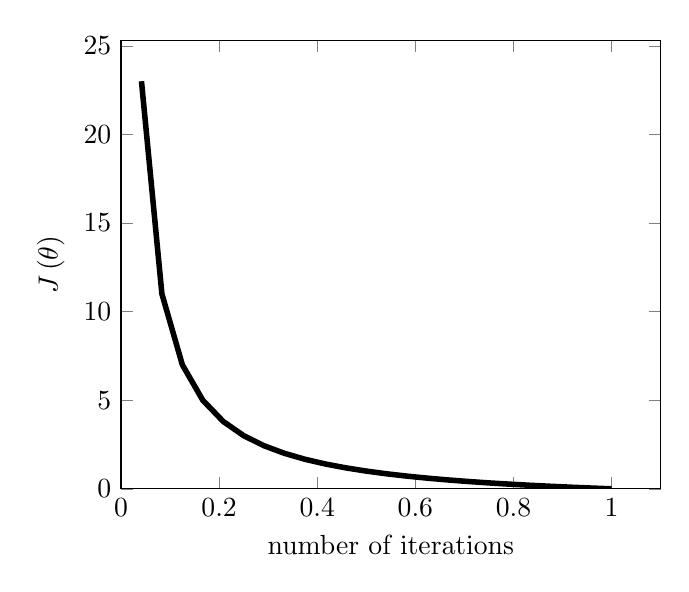
\begin{tikzpicture}
  \begin{axis}[
	domain=0:1,
	xmin=0,
	ymin=0,
    xlabel=number of iterations,
    ylabel={$J \left( \theta \right)$}    
  ] 
    \addplot[color=black, line width=2] {1/x - 1}; 
  \end{axis}
\end{tikzpicture}
\item If gradient descent is not working, use smaller \textcolor{OliveGreen}{$\alpha$}.
\item Typical values of \textcolor{OliveGreen}{$\alpha$}: \textcolor{OliveGreen}{$\alpha \leq 1$}, typically \textcolor{OliveGreen}{$0.01 \leq \alpha \leq 0.1$}. Hopefully.
\item If size of a vector is less than 1000 then normal equation (matrix inverse) is preferred over the gradient descent.
\item How to reduce the error:
\begin{itemize}
\item[--] reduce number of features;
\item[--] regularisation.
\end{itemize}
\item Regularisation parameter, \textcolor{OliveGreen}{$\lambda$}, should not be too large.
\end{enumerate}
\subsection{Classification}
\begin{enumerate}
\item Make sure that multiclasses in a Neural Network are defined as \textcolor{OliveGreen}{$\left[0, 1 \right]$} vectors.
\item Reasonable default architecture: 1 hidden layer or equal number of units in each layer if the number of layers is greater than 1.
\item Plotting \textcolor{OliveGreen}{$J \left( \theta \right)$} vs the number of iterations and making sure it doesn't increase helps.
\item One can evaluate a hypothesis by calculating \textcolor{OliveGreen}{$J \left( \theta \right)$} for a test set with parameters learned from the training set.
\item If a learning algorithm is suffering from high variance, then getting more data is likely to help. This can be learned from the gap between \textcolor{OliveGreen}{$J_{cv} \left( \theta \right)$} and \textcolor{OliveGreen}{$J_{train} \left( \theta \right)$} on the learning curves plot.
\item If a number of features, \textcolor{OliveGreen}{$n$}, is large comparing to the number of training examples, \textcolor{OliveGreen}{$m$}, use logistic regression, if \textcolor{OliveGreen}{$n$} is small, \textcolor{OliveGreen}{$m$} is intermediate -- use SVM with Gaussian kernel, if \textcolor{OliveGreen}{$n$} is small, \textcolor{OliveGreen}{$m$} is large -- create/add more features. A NN most likely would work better, but slower anyway.
\item Activation function \textcolor{OliveGreen}{$g(z) = \tanh (z)$} works almost always better than a sigmoid. Except for a binary classifier's output layer.
\item A good default activation function for hidden layer is \textit{ReLU}. \textit{Leaky ReLU} might be also used sometimes. It's much faster than \textcolor{OliveGreen}{$\tanh$}.
\item For a neural net one must initialise all the weights randomly, not to \textcolor{OliveGreen}{$0$} as it was acceptable for a logistic regression. This is required in order to prevent hidden layers from being linearly dependent.
\end{enumerate}
\subsection{Bias vs Overfitting}
Bias vs overfit:
\begin{itemize}
\item \textcolor{Red}{Bias} (underfit): \textcolor{OliveGreen}{$J_{train} \left( \theta \right) \rightarrow \text{high}$}, \textcolor{OliveGreen}{$J_{cv} \left( \theta \right) \approx J_{train} \left( \theta \right)$};
\item \textcolor{Green}{Variance} (overfit): \textcolor{OliveGreen}{$J_{train} \left( \theta \right) \rightarrow \text{low}$}, \textcolor{OliveGreen}{$J_{cv} \left( \theta \right) \geq J_{train} \left( \theta \right)$} .
\end{itemize}

Also one may also analyse learning curves.

In order to fix high \textcolor{Red}{bias} one may:
\begin{itemize}
\item try additional features or bigger network;
\item try adding polynomial features (regression only);
\item tune layers (nn only);
\item switch architecture (nn only);
\item try decreasing \textcolor{OliveGreen}{$\lambda$};
\item try better optimisation algorithm.
\end{itemize}

In order to fix high \textcolor{Green}{variance}:
\begin{itemize}
\item get more training examples (data);
\item try smaller set of features (regression only);
\item switch architecture (nn only);
\item try increasing \textcolor{OliveGreen}{$\lambda$}.
\end{itemize}

\subsection{Clustering}
\begin{enumerate}
\item Use ``elbow'' method to deduce how many clusters one needs. If there is a clear ``elbow''.
\item Other way of choosing the number of clusters might be relying on the nature of the problem. But there is no universal algorithm.
\end{enumerate}
\subsection{PCA}
\begin{enumerate}
\item Always perform feature scaling / mean normalisation before doing dimensionality reduction / PCA.
\item Applying PCA for a supervised learning algorithm, one should apply it for a training set only.
\item Bad use of PCA: overfitting prevention.
\end{enumerate}
\subsection{Anomaly Detection}
\begin{itemize}
\item For a skewed system with many negative examples and few positive examples it might be better to use anomaly detection. Also for many different reasons or types of anomalies. Should have definitely applied this to EY Brain.
\item Try to transform non-gaussian features for anomaly detection with log, sqrt or something similar to make them gaussian.
\item If anomaly detection algorithm performs poorly, then coming up wiht more features that distinguish between normal and anomalous examples may help.
\end{itemize}

\section{Questions}
\begin{enumerate}
\item Which minimisers do scikit-learn regression algorithms use?\\
\textbf{A:} It's ADAM usually.
\item Is scaling already implemented in multilinear regression in scikit-learn?\\
\textbf{A:} There's an option to control this.
\item Can mean normalisation be implemented in scikit-learn regression? Should it be always implemented?\\
\textbf{A:} Yes and mostly yes.
\item Do scikit-learn models support polynomial models in oppose to linear? Or any other custom models like \textcolor{OliveGreen}{$\sqrt{x}$}.\\
\textbf{A:} Yes. There is a \texttt{Polynomial} module.
\item Where does the expression of \textcolor{OliveGreen}{$\delta^{(l-1)}$} come from?
\item Can I derive all the \textcolor{OliveGreen}{$J \left( \theta \right)$} and its derivative in a proper tensor form with Einstein summation convention applied.
\item Is it true that some layers of a NN can be biased and some -- not?
\item What's Mercer's theorem?
\item Might be worth to build a proper block algorithm on how to approach a ML problem.
\item Can dimensionality reduction be applied to regression problems? Time series, namely.
\item Can I have Fourier Transform as an activation layer?
\end{enumerate}

\section{Critics}
\begin{enumerate}
\item Most of the mathematical derivations are mathematically inaccurate and insufficient.
\item Fucking Octave! Who codes in Octave these days?
\item Clustering and whatever comes after it is poorly covered.
\end{enumerate}

\end{document}